\subsection{Experimental Procedure}\label{subsec:experimental-procedure}

The object of the current investigation is the operation of the experimental semi-continuous rolling plant located at the Institute of Metal Forming, TU Bergakademie Freiberg.
It consists of a two-high reversing roughing stand and four continuous finishing stands.
The pass schedule of the current work consists of 10 oval-round reversing passes followed by 4 oval-round continuous finishing passes.
A \qty{50}{\milli\meter} round workpiece made of a mild structural steel is rolled down to \qty{8}{\milli\meter} diameter.
Details of the schedule are provided in \autoref{tab:process_conditions} and \autoref{tab:in_profile}, as well as in the supplemental material~\cite{WeinerVariationSupplemental2023}.
The supplemental material includes the whole code for data processing and simulation needed to reproduce the results of this work.

\begin{figure}
    \centering
    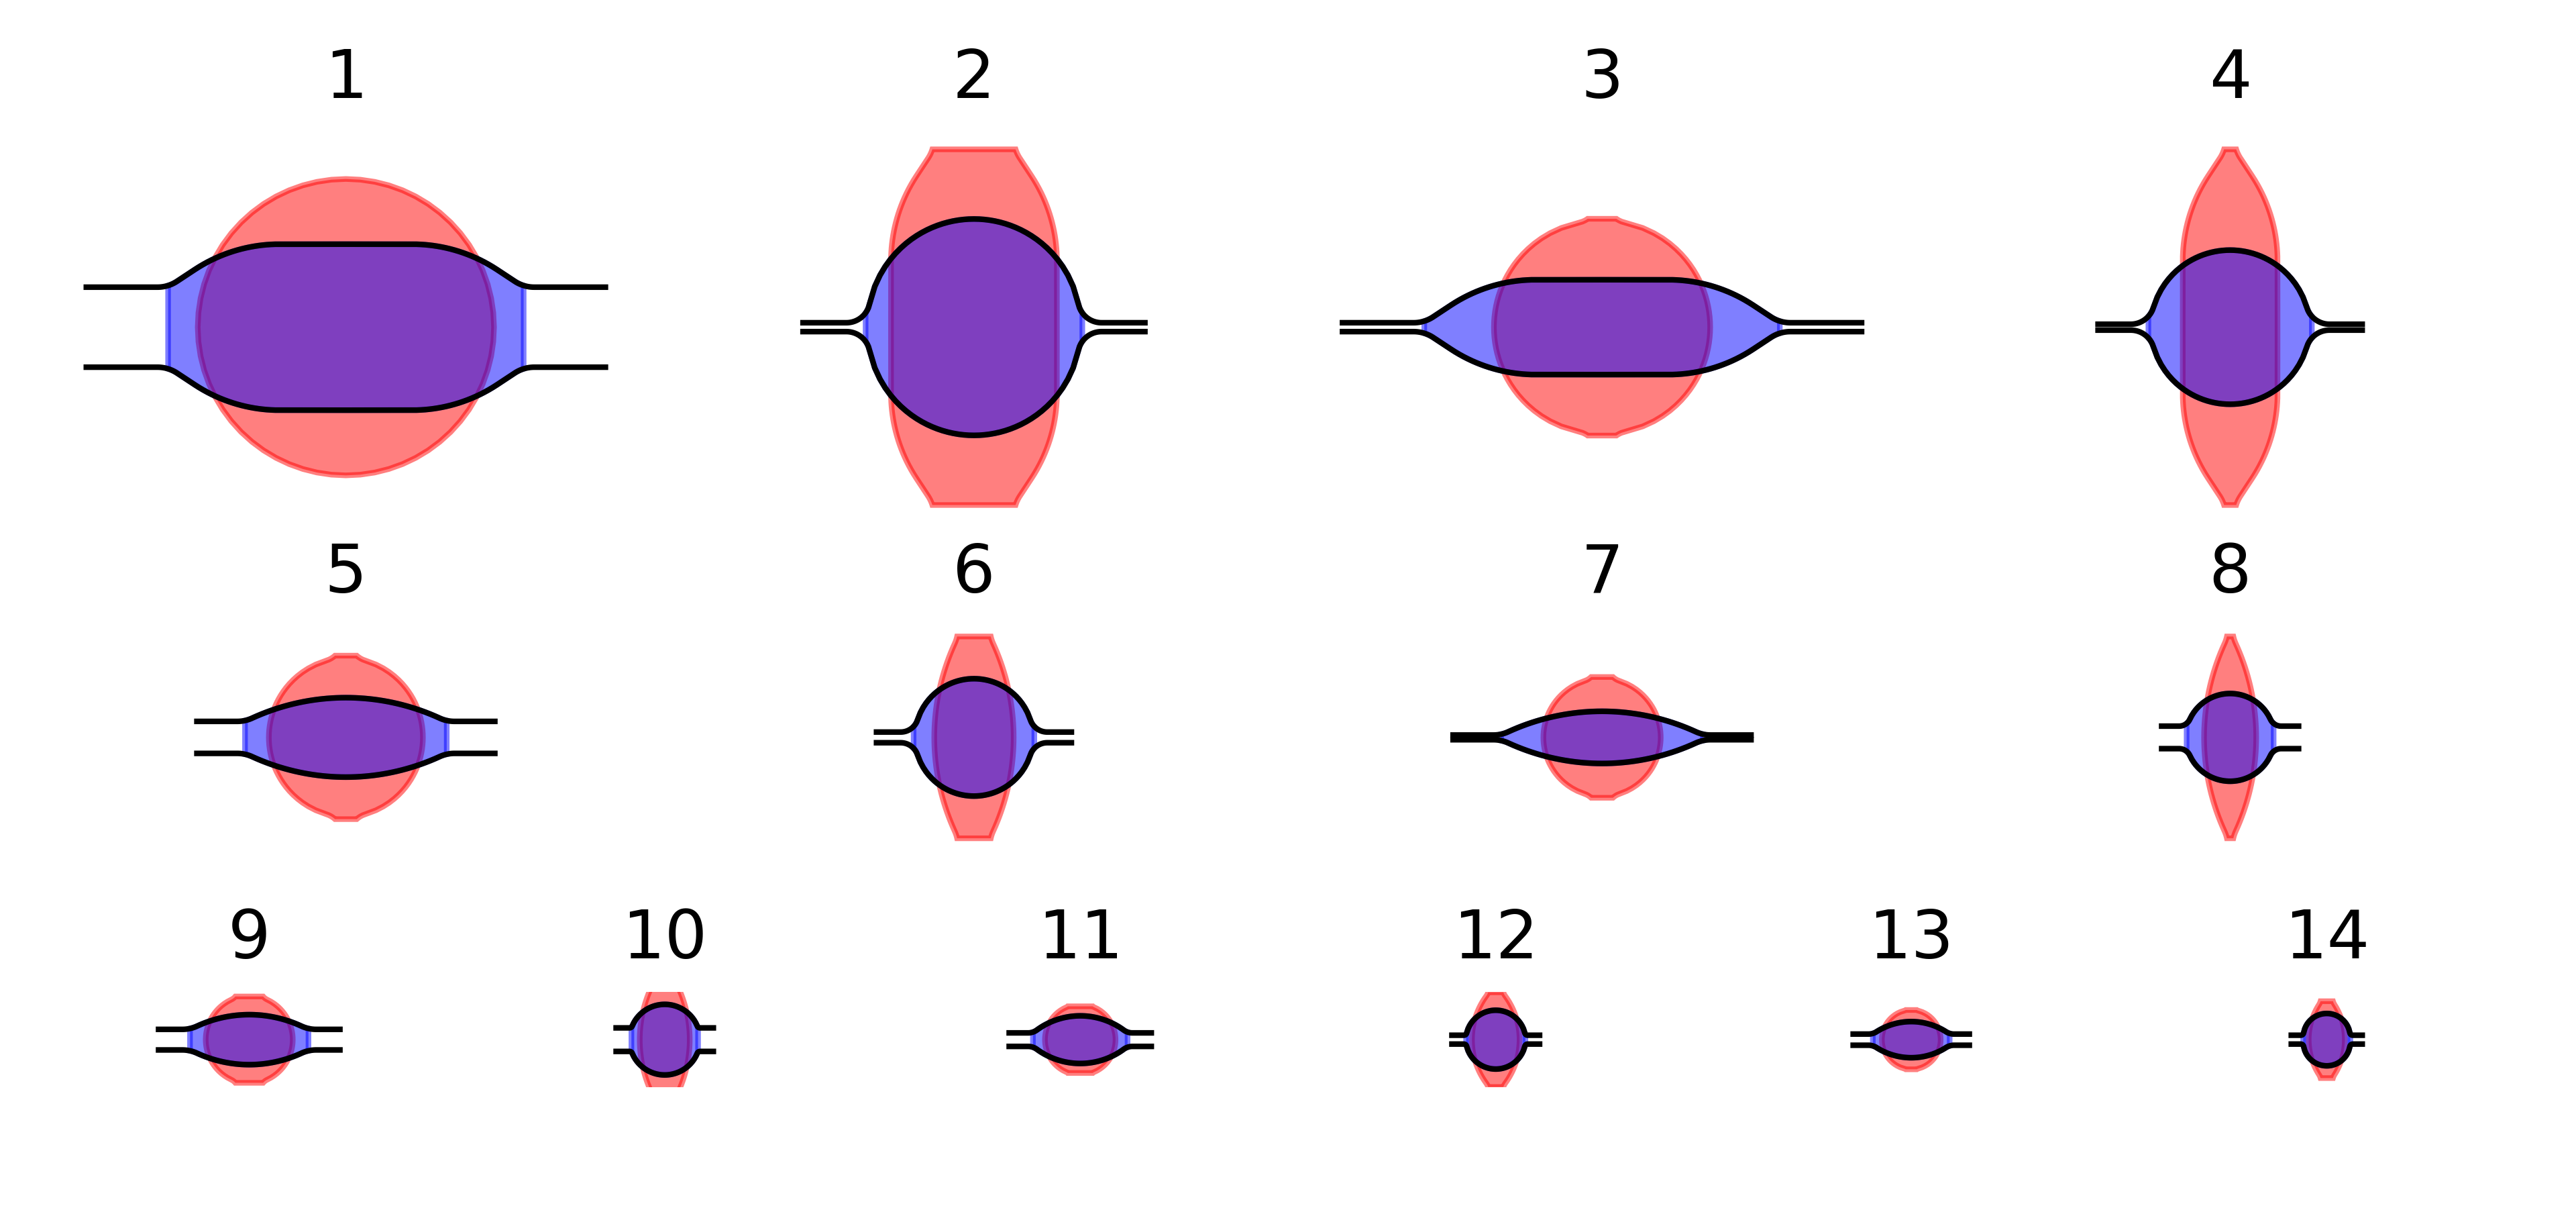
\includegraphics{img/plot_pass_sequence}
    \caption{True Scaled Illustration of the Investigated Pass Sequence}
    \label{fig:plot_pass_sequence}
\end{figure}


\begin{table}
    \centering
    \caption{Principal Data of the Investigated Pass Sequence}
    \label{tab:process_conditions}
    \begin{tblr}{colspec={l|XXXXXX}}
    \toprule
    \#             & Type                       & $\Width$                                               & $\Height$                                              & $\RollGap$                              & $\RollRadius$                                           & $\Velocity$                          \\
    &                            & \unit{\milli\meter}                                    & \unit{\milli\meter}                                    & \unit{\milli\meter}                     & \unit{\milli\meter}     & \unit{\meter\per\second}   \\
    \midrule
    
    {{ p.label }} & {{ p | format_pass_type }} & \num{ {{- (p.out_profile.width * 1e3) | round(1) -}} } & \num{ {{-  (p.out_profile.height * 1e3) | round(1) -}} } & \num{ {{-  (p.gap * 1e3) | round(1) -}} } & \num{ {{-  (p.roll.nominal_radius * 1e3) | round(1) -}} } & \num{ {{-  p.velocity | round(1) -}} }\\
    
    \bottomrule
\end{tblr}
\end{table}



\begin{table}
    \centering
    \caption{Principal Data of the Input Workpiece}
    \label{tab:in_profile}
    \begin{tblr}{
    colspec={XXXX},
    columns={r},
    row{1-2}={l},
}
        \toprule
        $\In\Diameter$ & $\In\Temperature$ & $\Density$ & $\ThermalCapacity$ \\
        \unit{\milli\meter} & \unit{\kelvin} & \unit{\kilo\gram\per\cubic\meter} & \unit{\joule\per\kilo\gram\per\kelvin} \\
        \midrule
        \num{ {{- (in_profile.height * 1e3) | round(1) -}} }  & \num{ {{- in_profile.temperature | round(1) -}} } & \num{ {{- in_profile.density | round(1) -}} } & \num{ {{- in_profile.thermal_capacity | round(1) -}} } \\
        \bottomrule
\end{tblr}
\end{table}

To achieve statistical certainty, about 50 rolling trials were performed.
A major source of variation in these trials is the manual feeding of the workpiece into the reversing passes.
The duration of those is scheduled with about 6 seconds.
The actual time needed has to be investigated in this work, see \autoref{subsec:data-acquisition} for details.

\subsection{Monte-Carlo Approach}\label{subsec:monte-carlo-approach}

\begin{figure}
    \centering
    \includegraphics[width=\linewidth]{img/chart_mc_principle}
    \caption{Chart of the Concept of Variation Estimation Using Monte Carlo Techniques}
    \label{fig:chart_mc_principle}
\end{figure}

The basic idea of the approach shown here is to simulate the rolling process several times with different input values, which are drawn by a random number generator according to predefined statistical distributions.
Afterwards, the distribution of the results can be analysed by classic methods of descriptive statistics to obtain information about the process' variational behavior.
The principle is shown in \autoref{fig:chart_mc_principle}.

This approach provides information about the overall variational behavior of the process.
If a single source of variation is introduced in the input, the reaction of the process on this variable can be analysed.
The count of variation sources introduced is generally unbounded.
In contrast to classic Taylor series error propagation, the computational effort does not directly increase remarkably with increasing count of investigated parameters.
However, an increase in sample size can be necessary to achieve sufficient certainty.
The tracing back of result variations to the input can be done using classic correlation methods of descriptive statistics, however, with the same typical caveats.
The main benefit of the approach is, that no information about the internals of the simulation procedure is needed for variational analysis, especially there is no need for derivatives of result values in dependence on the input.
The simulation procedure can generally be treated as black box with defined input and output interfaces.

The key problem is to obtain data describing the variations of the input variables.
In this work two showcases shall be regarded: first the variation of the initial workpiece in diameter and temperature,
second the variation of the inter-pass durations between the reversing passes.
This choice was taken, since two fundamentally different types of variation sources were suspected.
First, sources in the initial workpiece, which are applied only once, but traverse the whole process line.
Second, variations in the process itself, which affect the workpiece state in each process step anew.

\subsection{Statistical Data Acquisition}\label{subsec:data-acquisition}

The pilot plant at IMF is equipped with several measurement and data collection systems.
Data from a number of rolling trials have been collected and analysed to obtain the interpass durations $\InterpassDuration$ between the reversing passes.
The complete dataset and analysis routines are available in the supplemental material~\cite{WeinerVariationSupplemental2023}.

The question of varying inter-pass durations is crucial for scientific experiments on microstructure evolution, but currently often neglected.
Mostly, only flat durations between the reversing passes are included in the design calculations.
Due to manual transport and feed of the workpiece to the following roll pass, the scheduled inter-pass durations are never realized in practice.
Although, these deviations from the schedule influence the microstructure evolution of the sample, as well as the actual conditions in the roll passes.
The current approach is aimed to help quantifying these deviations.

To obtain the pause durations from the timeline data, the passes have to be identified automatically.
This is done by analysing the roll torque signal as plotted in \autoref{fig:plot_timeline_pass_finding}.
The original signal is first downsampled and smoothed.
Then, a difference filter is applied and the peaks of the resulting signal are determined.
These peaks denote start and end times of the roll passes, the middle time of those is used as time coordinate of the roll pass.
The distances of those are used as the inter-pass durations.

\begin{figure}
    \centering
    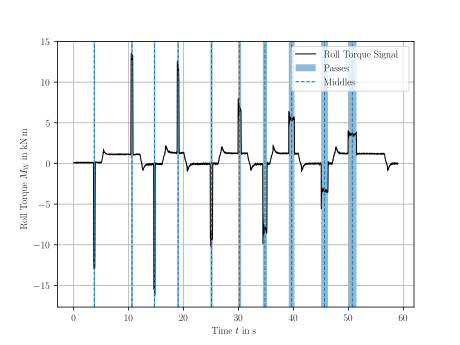
\includegraphics{img/plot_timeline_pass_finding}
    \caption{Example Roll Torque Signal With Automatically Determined Roll Pass Locations}
    \label{fig:plot_timeline_pass_finding}
\end{figure}


For the approximative description of the durations' distribution, a gamma distribution was used, which is a generalized exponential distribution.
The probability density function (PDF) of the gamma distribution is defined as in \autoref{eq:gamma-dist}, where $\Gamma$ is the gamma function and $\GammaDistributionAlpha > 0$ and $\GammaDistributionBeta > 0$ are parameters.

\begin{equation}
    f(x) = \frac{\GammaDistributionBeta^\GammaDistributionAlpha}{\Gamma(\GammaDistributionAlpha)}x^{\GammaDistributionAlpha - 1} \exp(-\GammaDistributionBeta x)
    \label{eq:gamma-dist}
\end{equation}

Since the gamma distribution is only defined for $x>0$, but no interpass durations below a certain value occur due to technical restrictions, the distribution was modified by introducing a minimal interpass duration $\MinInterpassDuration$ with $x = \InterpassDuration - \MinInterpassDuration$.
So there are three free parameters $\GammaDistributionAlpha$, $\GammaDistributionBeta$ and $\MinInterpassDuration$ for fitting of the distribution function.
The fitting is done using least squares optimization of the resulting PDF function on the density histogram of the data.

Regarding the geometric variations of the input workpiece, the diameter of the samples was determined at multiple spots using a calibre.
The initial temperature of the samples was determined using the pyrometer installed near the roll gap entry.

\subsection{Core Simulation Procedure}\label{subsec:simulation-procedure}

In the current work, the open-source rolling simulation framework PyRolL~\cite{pyroll2} was used to simulate the rolling process.
Generally, the shown approach can be used with every rolling simulation software available, since the procedure does not depend on any internals of the simulation.
A fast simulation approach, however, is favourable, since the simulation has to be done several, up to hundreds of, times.
The models used here are of one-dimensional type, thus, they lack of resolution in other directions as the rolling direction and provide only limited accuracy, but at the benefit of high solution speed.
They typically combine empirical approaches with simplified analytical solutions.
The simulation was done with the basic configuration of PyRolL, which includes the empirical roll force and torque model of \textcite{Hensel1978}, an integral thermal model approach according to \textcite{Hensel1990}, contact area estimation according to \textcite{Zouhar1960} and roll flattening according to \textcite{Hitchcock1935}.
Spreading was simulated using the equivalent flat pass according to \citeauthor*{Lendl1948}~\cite{Lendl1948, Lendl1948a, Lendl1949} in conjunction with the spreading equation of \textcite{Wusatowski1969}.
Details of software construction and model equations are provided in the documentation of PyRolL~\cite{pyroll}.

The object of the current investigation is the operation of the experimental semi-continuous rolling plant located at the Institute of Metal Forming, TU Bergakademie Freiberg.
The process consists of several reversing passes and up to four continuous finishing passes.
The feeding in the reversing passes is done manually, so there is an obvious source of variation in process, since the human operator can not achieve precisely a defined duration between the passes.
In this work the evolution of variation regarding temperature and microstructure state


